\section{Problema 3: El se\~nor de los caballos}
\subsection{Descripci\'on de la problem\'atica}

En este problema, se presenta un tablero de ajedrez de tama\~no $nxn$, el cual cuenta con alguna cantidad de caballos ubicados en una posici\'on aleatoria del tablero. Lo que se quiere lograr es \emph{cubrir} todo el tablero. Un casillero se considera cubierto si hay un caballo en \'el o bien, si es una posici\'on en la cual alg\'un caballo existente puede moverse con un s\'olo movimiento. Para lograr este cometido, puede ser necesario agregar nuevas fichas \emph{caballo} al tablero. No existe un l\'imite en la cantidad de caballos para agregar, pero lo que se busca es dar una soluci\'on agregando la m\'inima cantidad de caballos posibles.\\


En la figura \ref{caballito} se pueden ver todas las casillas que est\'an cubiertas por un s\'olo caballo.


 \begin{figure}[h!]
   \begin{center}
 	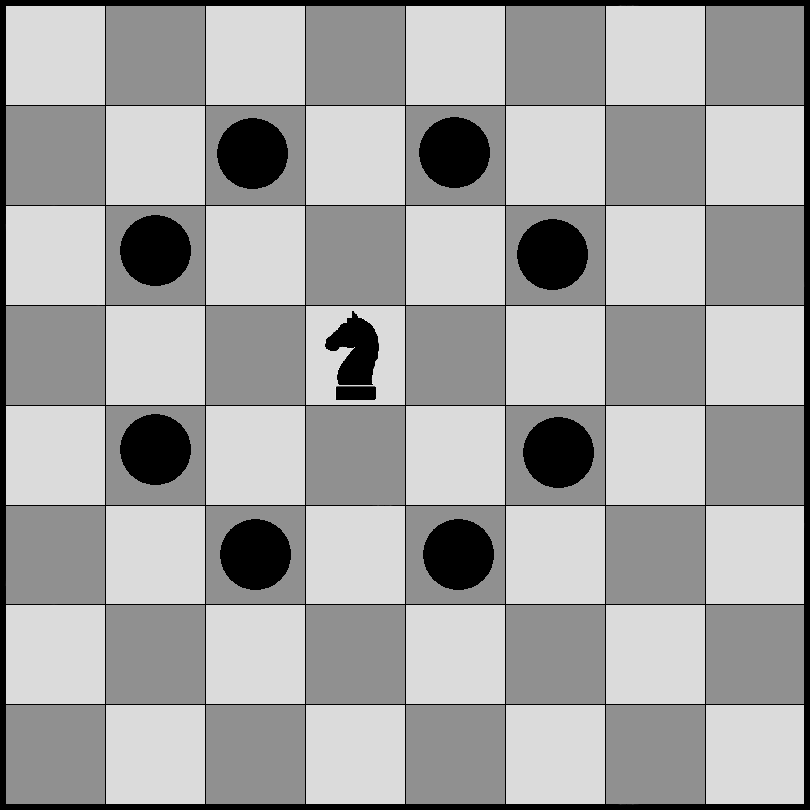
\includegraphics[scale=0.3]{imagenes/ej3/caballito.png}
 	\caption{Casillas que \emph{cubre} un caballo}
 	\label{caballito}	
   \end{center}
 \end{figure}



\newpage
\subsection{Resoluci\'on propuesta y justificaci\'on}
Para la resoluci\'on de este ejercicio, se ped\'ia un algoritmo de backtracking. La soluci\'on que presentamos tiene inclu\'idas estrategias para que el algoritmo resuelva en un tiempo razonable los problemas medianos.\\

Simplemente se fija cu\'antos caballos necesita colocar para cubrir el tablero si no coloca un caballo en alguna posici\'on y luego se fija cu\'antos har\'an falta si lo pone en la misma posici\'on.\\

\newpage

\subsection{An\'alisis de la complejidad}
Para analizar la complejidad de este algoritmo, hay que tener en cuenta algunas situaciones. Si el tablero viene cubierto por los caballos preubicados, entonces el algoritmo chequea esto y devuelve que est\'a completo en tiempo $O(n^{2})$. Si no empieza a trabajar con el backtracking.\\

El primer approach para la resoluci\'on del ejercicio fue aplicar "fuerza bruta", d\'andonos una complejidad de $O(2^{n^{2} - k})$ siendo n la dimensi\'on del tablero y k la cantidad de caballos preubicados. Esto es para cada posici\'on sin caballos, ver que pasa si tomo alguna de las dos posibles decisiones.\\

Para disminuir esta cota de complejidad, se plantearon podas y estrategias, es decir, determinar si vale la pena o no seguir revisando alguna rama del \'arbol de soluciones que propone esta t\'ecnica de programaci\'on.\\

La primera poda fue la m\'as intuitiva, si tenemos una soluci\'on con k caballos extra agregados,  y analizando otra rama llegamos a tener que necesitar agregar un caballo a una subsoluci\'on de k-1 caballos (o sea que tendr\'ia por lo menos k caballos), entonces no nos interesa seguir revisandola, pues tenemos una soluci\'on que es igual o m\'as \'optima con k caballos.\\

La segunda estrategia fue plantear si en alg\'un momento sab\'iamos que deb\'iamos agregar o no un caballo en un determinado casillero. Entonces, salteamos la disyuntiva de las k posiciones de los caballos preubicados y adem\'as salteamos aquellas posiciones que, estando atacadas, si le pusieramos un caballo, estar\'ian atancando a casilleros que ya est\'an siendo atacados por otros caballos.\\

Ninguna poda/estrategia disminuye la complejidad te\'orica exponencial del primer approach, dado que el algoritmo realiza las mismas preguntas para cada posici\'on del tablero, ¿qu\'e pasa si lo dejo sin caballo? ¿qu\'e pasa si le pongo un caballo?. No obstante, los tiempos de ejecuci\'on se ven radicalmente afectados, esto sucede porque se poda el \'arbol de soluciones posibles que se analizan, es decir, en el primer approach, se revisan todas las ramas, sin excepci\'on, y aplicando podas descartamos muchas de estas que ya sabemos que no nos llevar\'an a un resultado que nos interese.\\
\newpage

\subsection{C\'odigo fuente}
\newpage
\subsection{Experimentaci\'on}

\subsubsection{Constrastaci\'on Emp\'irica de la complejidad}
-Hacer lo que hicieron en clase\\
\newpage
